\documentclass[crop, tikz]{standalone} 
\usetikzlibrary{calc,positioning,shapes,decorations.pathmorphing}

\begin{document}
    \begin{tikzpicture}[remember picture]
        %% Graph 1 (V,E)
    	\node[circle, thick, draw] (0) {\tiny $\vec{h}_a$};
    	\node[circle, thick, draw, above right=0.1em and 3em of 0] (1) {\tiny $\vec{h}_b$};
    	\node[circle, thick, draw, above right=0.8em and 0.5em of 0] (2) {\tiny $\vec{h}_c$};
    	\node[circle, thick, draw, left=of 0] (3) {\tiny $\vec{h}_d$};
    	\node[circle, thick, draw, below left=0.8em and 1.5em of 0] (4) {};
    	
    	\draw[-, thick] (0) -- (1);
    	\draw[-, thick] (0) -- (2);
    	\draw[-, thick] (0) -- (3);
    	\draw[-, thick] (4) -- (3);
    	
    	\node[rectangle, draw, dashed, minimum width=12.4em, minimum height=6em, yshift=0.4em, xshift=-0.2em] (RR) {};
    	\node[below=0em of RR] (l1) {$({\bf H}, {\bf E})$};
        \begin{lrbox}{0}
        \begin{scope}
    	    %% Message passing
    	    \draw[->, line width=0.5mm, color=cyan!70!black] (1) -- (0);
        	\draw[->, line width=0.5mm, color=cyan!70!black] (2) -- (0);
        	\draw[->, line width=0.5mm, color=cyan!70!black] (3) -- (0);
        	\draw[->, line width=0.5mm, color=cyan!70!black] (3) -- node[above] {$M(\cdot)$} (0);
        	
        	\path[draw,line width=5pt,-,cyan!70!black, opacity=0.4] (1) -- (0);
        	\path[draw,line width=5pt,-,cyan!70!black, opacity=0.4] (2) -- (0);
        	\path[draw,line width=5pt,-,cyan!70!black, opacity=0.4] (3) -- (0);
        	
        	\node[circle, ultra thick, draw, draw=cyan!70!black, text opacity=0] (m1) at ($(0)$) {\tiny $\vec{h}_i$};
    	    %% Graph 2 (V,E)
    	    \node[rectangle, draw, dashed, minimum width=11.5em, minimum height=6em, right=10.25em of 0,yshift=0.4em] (RR) {};
    	    \node[below=0em of RR] (l1) {$({\bf H'}, {\bf E})$};
    	    
        	\node[circle, thick, draw, right=15em of 0,draw=green!70!black] (01) {\tiny $\vec{h}'_a$};
        	\node[circle, thick, draw, above right=0.1em and 3em of 01] (1) {};
        	\node[circle, thick, draw, above right=0.8em and 0.5em of 01] (2) {};
        	\node[circle, thick, draw, left=of 01] (3) {};
        	\node[circle, thick, draw, below left=0.8em and 1.5em of 01] (4) {};
        	
        	\draw[-, thick] (01) -- (1);
        	\draw[-, thick] (01) -- (2);
        	\draw[-, thick] (01) -- (3);
        	\draw[-, thick] (4) -- (3);
        	
        	%% GNN connector
            \draw[-stealth, very thick, decoration={snake, pre length=0.01mm, segment length=2mm, amplitude=0.3mm, post length=1.5mm}, decorate,color=green!70!black] (0) to[out=90,in=90] node[above] {$U(\cdot)$} (01);
        \end{scope}
        \end{lrbox}
    \end{tikzpicture}

    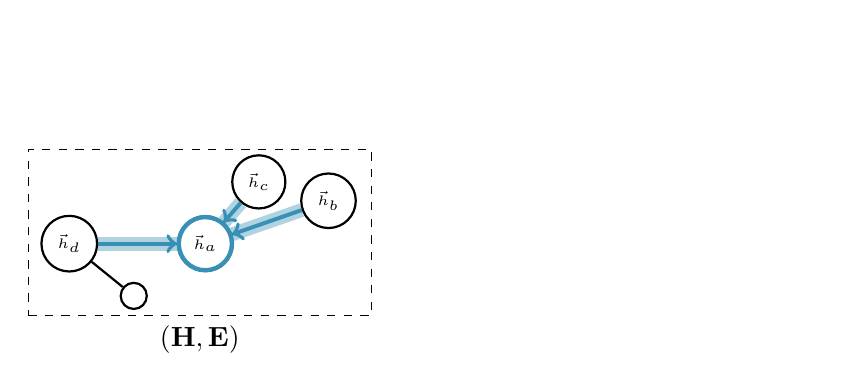
\begin{tikzpicture}[remember picture]
        %% Graph 1 (V,E)
    	\node[circle, thick, draw] (0) {\tiny $\vec{h}_a$};
    	\node[circle, thick, draw, above right=0.1em and 3em of 0] (1) {\tiny $\vec{h}_b$};
    	\node[circle, thick, draw, above right=0.8em and 0.5em of 0] (2) {\tiny $\vec{h}_c$};
    	\node[circle, thick, draw, left=of 0] (3) {\tiny $\vec{h}_d$};
    	\node[circle, thick, draw, below left=0.8em and 1.5em of 0] (4) {};
    	
    	\draw[-, thick] (0) -- (1);
    	\draw[-, thick] (0) -- (2);
    	\draw[-, thick] (0) -- (3);
    	\draw[-, thick] (4) -- (3);
    	
    	\node[rectangle, draw, dashed, minimum width=12.4em, minimum height=6em, yshift=0.4em, xshift=-0.2em] (RR) {};
    	\node[below=0em of RR] (l1) {$({\bf H}, {\bf E})$};
        %% Message passing
        \draw[->, line width=0.5mm, color=cyan!70!black] (1) -- (0);
        \draw[->, line width=0.5mm, color=cyan!70!black] (2) -- (0);
        \draw[->, line width=0.5mm, color=cyan!70!black] (3) -- (0);
        
        \path[draw,line width=5pt,-,cyan!70!black, opacity=0.4] (1) -- (0);
        \path[draw,line width=5pt,-,cyan!70!black, opacity=0.4] (2) -- (0);
        \path[draw,line width=5pt,-,cyan!70!black, opacity=0.4] (3) -- (0);
        
        \node[circle, ultra thick, draw, draw=cyan!70!black, text opacity=0] (m1) at ($(0)$) {\tiny $\vec{h}_i$};
        \begin{lrbox}{0}
        \begin{scope}
    	    %% Graph 2 (V,E)
    	    \node[rectangle, draw, dashed, minimum width=11.5em, minimum height=6em, right=10.25em of 0,yshift=0.4em] (RR) {};
    	    \node[below=0em of RR] (l1) {$({\bf H'}, {\bf E})$};
    	    
        	\node[circle, thick, draw, right=15em of 0,draw=green!70!black] (01) {\tiny $\vec{h}'_a$};
        	\node[circle, thick, draw, above right=0.1em and 3em of 01] (1) {};
        	\node[circle, thick, draw, above right=0.8em and 0.5em of 01] (2) {};
        	\node[circle, thick, draw, left=of 01] (3) {};
        	\node[circle, thick, draw, below left=0.8em and 1.5em of 01] (4) {};
        	
        	\draw[-, thick] (01) -- (1);
        	\draw[-, thick] (01) -- (2);
        	\draw[-, thick] (01) -- (3);
        	\draw[-, thick] (4) -- (3);
        	
        	%% GNN connector
            \draw[-stealth, very thick, decoration={snake, pre length=0.01mm, segment length=2mm, amplitude=0.3mm, post length=1.5mm}, decorate,color=green!70!black] (0) to[out=90,in=90] node[above] {$U(\cdot)$} (01);
        \end{scope}
        \end{lrbox}
    \end{tikzpicture}

    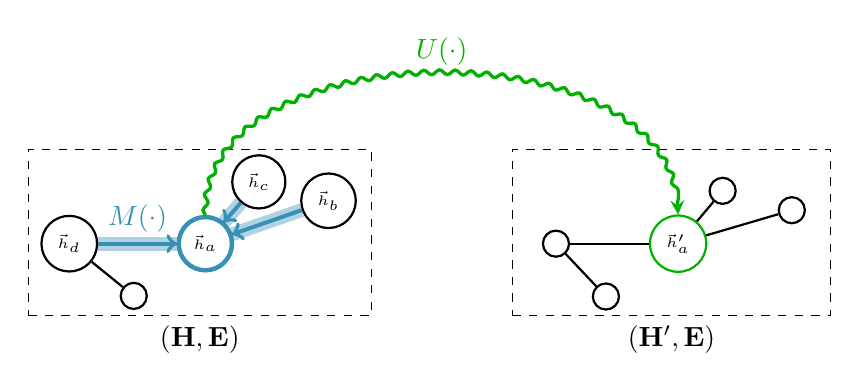
\begin{tikzpicture}[remember picture]
        %% Graph 1 (V,E)
    	\node[circle, thick, draw] (0) {\tiny $\vec{h}_a$};
    	\node[circle, thick, draw, above right=0.1em and 3em of 0] (1) {\tiny $\vec{h}_b$};
    	\node[circle, thick, draw, above right=0.8em and 0.5em of 0] (2) {\tiny $\vec{h}_c$};
    	\node[circle, thick, draw, left=of 0] (3) {\tiny $\vec{h}_d$};
    	\node[circle, thick, draw, below left=0.8em and 1.5em of 0] (4) {};
    	
    	\draw[-, thick] (0) -- (1);
    	\draw[-, thick] (0) -- (2);
    	\draw[-, thick] (0) -- (3);
    	\draw[-, thick] (4) -- (3);
    	
    	\node[rectangle, draw, dashed, minimum width=12.4em, minimum height=6em, yshift=0.4em, xshift=-0.2em] (RR) {};
    	\node[below=0em of RR] (l1) {$({\bf H}, {\bf E})$};
    	    %% Message passing
    	    \draw[->, line width=0.5mm, color=cyan!70!black] (1) -- (0);
        	\draw[->, line width=0.5mm, color=cyan!70!black] (2) -- (0);
        	\draw[->, line width=0.5mm, color=cyan!70!black] (3) -- node[above] {$M(\cdot)$} (0);
        	
        	\path[draw,line width=5pt,-,cyan!70!black, opacity=0.4] (1) -- (0);
        	\path[draw,line width=5pt,-,cyan!70!black, opacity=0.4] (2) -- (0);
        	\path[draw,line width=5pt,-,cyan!70!black, opacity=0.4] (3) -- (0);
        	
        	\node[circle, ultra thick, draw, draw=cyan!70!black, text opacity=0] (m1) at ($(0)$) {\tiny $\vec{h}_i$};
    	    %% Graph 2 (V,E)
    	    \node[rectangle, draw, dashed, minimum width=11.5em, minimum height=6em, right=10.25em of 0,yshift=0.4em, xshift=-0.2em] (RR) {};
    	    \node[below=0em of RR] (l1) {$({\bf H'}, {\bf E})$};
    	    
        	\node[circle, thick, draw, right=15em of 0,draw=green!70!black] (01) {\tiny $\vec{h}'_a$};
        	\node[circle, thick, draw, above right=0.1em and 3em of 01] (1) {};
        	\node[circle, thick, draw, above right=0.8em and 0.5em of 01] (2) {};
        	\node[circle, thick, draw, left=of 01] (3) {};
        	\node[circle, thick, draw, below left=0.8em and 1.5em of 01] (4) {};
        	
        	\draw[-, thick] (01) -- (1);
        	\draw[-, thick] (01) -- (2);
        	\draw[-, thick] (01) -- (3);
        	\draw[-, thick] (4) -- (3);
        	
        	%% GNN connector
            \draw[-stealth, very thick, decoration={snake, pre length=0.01mm, segment length=2mm, amplitude=0.3mm, post length=1.5mm}, decorate,color=green!70!black] (0) to[out=90,in=90] node[above] {$U(\cdot)$} (01);
    \end{tikzpicture}


\end{document}
